\documentclass[conference]{IEEEtran}
\usepackage[utf8]{inputenc}
\usepackage[T5]{fontenc}
\usepackage{cite}
\usepackage{amsmath,amssymb}
\usepackage{graphicx}
\usepackage{booktabs,array}
\usepackage{balance}
\usepackage{url}
\usepackage[hidelinks]{hyperref}
\graphicspath{{BaoCao/image_result/}}
\newcommand{\CE}{\operatorname{CE}}
\newcommand{\KL}{\operatorname{KL}}
% Fixed type size for all tables; fit columns without scaling the text.
\newcommand{\reporttablefont}{\normalfont\small}

\begin{document}
\title{Evaluating Boundary Unlearning on CIFAR-10 and CIFAR-100}
\author{\IEEEauthorblockN{Nguyễn Viết Hòa, Nguyễn Quang Khải, Nguyễn Tiến Nhật}
\IEEEauthorblockA{Faculty of Mathematics and Computer Science\\
University of Science\\
Vietnam National University, Ho Chi Minh City}}
\maketitle
\begin{abstract}
Machine unlearning aims to remove the influence of data requested for deletion from a trained model. However, retraining a model from scratch on the remaining data is often costly in terms of time and computational resources. Boundary Unlearning addresses this problem by shifting decision boundaries to alter predictions on the class to be forgotten while limiting the impact on the retained classes. This study evaluates Boundary Shrink and Boundary Expanding and investigates enhanced Boundary Shrink configurations that combine boundary-crossing threshold search, pseudo-label confidence weighting, and knowledge distillation from a pretrained model. The methods are compared with Original and Retrain models on CIFAR-10 and CIFAR-100, while the enhanced configurations are evaluated on CIFAR-10 only. The results show that Boundary Shrink and Boundary Expanding reduce recognition accuracy on the forgotten class but degrade performance on the retained classes. The enhanced configurations recover part of the retained-class performance at a higher computational cost.
\end{abstract}
\begin{IEEEkeywords}
Machine Unlearning, Class Unlearning, Boundary Shrink, Boundary Expanding, CIFAR-10, CIFAR-100, Knowledge Distillation.
\end{IEEEkeywords}

\section{Introduction}
As data are increasingly used to train machine learning models, removing data from models that have already been trained has attracted growing attention. Deleting data from storage alone does not remove their influence from a trained neural network. Machine unlearning addresses this problem by updating models to reduce the influence of data requested for removal, in response to data governance and privacy requirements~\cite{bourtoule2021machine}. A common reference approach is to retrain a model from scratch on the dataset after removing the designated samples. Although this approach provides a basis for comparison, it requires substantial computational resources and training time. A machine unlearning method is therefore evaluated along three main dimensions: reducing the influence of the data to be forgotten, preserving performance on the remaining data, and limiting computational cost.

Boundary Unlearning, proposed by Chen et al.~\cite{chen2023boundary}, modifies decision boundaries through two mechanisms: Boundary Shrink and Boundary Expanding. We adopt these two methods and extend Boundary Shrink using Weight Assign, then compare and evaluate their performance.

The study has two parts. First, we compare the same four models---Original, Retrain, Boundary Shrink, and Boundary Expanding---on CIFAR-10 and CIFAR-100. Second, we investigate two enhanced Boundary Shrink variants on CIFAR-10 only. The evaluation examines the reduction in forgotten-class accuracy and the loss of retained-class accuracy relative to Retrain, together with computational cost under two settings with different forget-set sizes. On CIFAR-10, we further investigate whether the two variants improve the trade-off between retained-class accuracy, forgotten-class accuracy, and execution time.

The contributions of this project are a comparison across two datasets, the implementation and evaluation of two Boundary Shrink variants on CIFAR-10, and an analysis of the trade-off between performance and computational cost.

\section{Related Work}
SISA~\cite{bourtoule2021machine} partitions training into shards to limit the influence of individual samples and reduce the amount of retraining required after deletion. This approach requires the data to be partitioned during the initial training stage. Another line of work modifies the weights of a trained model, as in selective forgetting~\cite{golatkar2020eternal}. The cost and quality of these methods depend on the approximations used and the experimental setting.

Boundary Unlearning~\cite{chen2023boundary} uses intuition about decision boundaries to design model updates. Visual observations motivate the algorithm, while forgetting quality is quantified through comparison with Retrain. This report evaluates Boundary Shrink and Boundary Expanding under a common experimental protocol.

The adopted components include FGSM~\cite{goodfellow2015explaining}, AllCNN~\cite{springenberg2015allcnn} with Batch Normalization~\cite{ioffe2015batch}, and knowledge distillation~\cite{hinton2015distilling}. Grad-CAM~\cite{selvaraju2017gradcam} and t-SNE~\cite{maaten2008tsne} provide additional qualitative analyses of model behavior after unlearning.
\section{Methods}

Let $D$ denote the training set, $D_f$ the forget set containing all samples from one class, and $D_r=D\setminus D_f$ the retain set. The corresponding test sets are denoted by $D_{ft}$ and $D_{rt}$. Original ($f_{w_0}$) is trained on $D$, whereas Retrain ($f_{w^*}$) is trained from scratch on $D_r$. Both retain $K$ outputs. Boundary Shrink and Boundary Expanding are the two adopted mechanisms for updating Original~\cite{chen2023boundary}.

\begin{figure}[!b]
\centering
\includegraphics[width=\linewidth]{\detokenize{paper_fig2_boundary_shrink_expanding.png}}
\caption{Principles of Boundary Shrink and Boundary Expanding, reproduced from Chen et al.~\cite{chen2023boundary}.}
\label{fig:boundary-methods}
\end{figure}

\subsection{Boundary Shrink}
Assigning random labels to samples in $D_f$ and continuing training can distort the boundaries of neighboring retained classes. Boundary Shrink addresses this problem through Neighbor Searching along an adversarial gradient direction.

For each forget sample $x_f \in D_f$ with original label $y$, a perturbed sample $x'_f$ is generated in the direction that increases the classification loss of the original model $f_{w_0}$:
\begin{equation}
x'_f = x_f + \epsilon \cdot \operatorname{sign}\!\left(\nabla_{x_f} \mathcal{L}(x_f,y,w_0)\right).
\end{equation}
In the implementation, perturbations are applied in pixel space, clipped to $[0,1]$, quantized to 8-bit values, and normalized before being passed to the network. With a fixed $\epsilon$, whether the boundary is crossed depends on the individual sample.

The perturbed sample $x'_f$ is then passed through the original model $f_{w_0}$ to obtain a new predicted label:
\begin{equation}
y_{nbi} \leftarrow \arg\max_k \operatorname{softmax}\!\left(f_{w_0}(x'_f)\right).
\end{equation}
The resulting label depends on the perturbation direction and magnitude and may coincide with the original label. The boundary-crossing rate is defined as the proportion of samples whose new predicted label differs from the original label.

The model is fine-tuned using the original images $x_f$ with the new target labels $y_{nbi}$:
\begin{equation}
w' = \arg\min_w \frac{1}{|D_f|}\sum_{(x_i,y_i)\in D_f} \CE(f_w(x_i),\widetilde y_i),
\end{equation}
where $\widetilde y_i=y_{nbi}(x_i)$ is the target label generated for each image. The updates aim to change predictions on the forgotten class according to these labels.

\subsection{Boundary Expanding}
To reduce the gradient computation required to generate boundary-crossing samples in Boundary Shrink, Boundary Expanding enlarges the class space by adding a neuron to the final classifier, increasing the output dimension from $K$ to $K+1$. The additional neuron represents a shadow class, denoted by $y_{shadow}$.

The expanded model is fine-tuned on the forget set $D_f$ with $y_{shadow}$ as the target label:
\begin{equation}
w'=\arg\min_w\frac{1}{|D_f|}\sum_{(x_i,y_i)\in D_f}\CE(f_w(x_i),y_{shadow}).
\end{equation}
This operation redirects activations associated with $D_f$ toward the additional neuron, reducing the response of the neuron originally representing the forgotten class.

After a small number of fine-tuning epochs, the $(K+1)$-th neuron is removed, returning the model to $K$ outputs. Predictions after pruning are obtained from the logits of the remaining outputs.


\subsection{Boundary Shrink with Weight Assign}

Boundary Shrink uses pseudo-labels to fine-tune the model on the original images, but the model being fine-tuned is not informed of the confidence associated with those pseudo-labels. When the probability of the selected class is only slightly higher than that of the second-ranked class, the prediction is ambiguous and the sample may lie near a decision boundary.

Weight Assign therefore uses the gap between these two probabilities to assign relatively larger weights to ambiguous samples and smaller weights to confident samples. Fine-tuning consequently places relatively greater emphasis on samples with ambiguous predictions.

In the \textit{Weight Assignment} variant, the frozen original model \(f_{\theta_0}\) predicts on the perturbed image \(x'_f\), producing the probability distribution

\[
p_i = \operatorname{softmax}(f_{\theta_0}(x'_f))
\]

and the pseudo-label

\[
\hat{y}_i = \arg\max_c p_{i,c}.
\]

Let \(p_i^{(1)} = p_{i,\hat{y}_i}\) be the highest probability and \(p_i^{(2)} = \max_{c\ne\hat{y}_i}p_{i,c}\) the second-highest probability. Their difference,

\[
PM_i = p_i^{(2)} - p_i^{(1)},
\]

is used to compute the weight

\[
w_i = 3\sigma\!\left(5(PM_i-0.5)\right),
\]

where \(\sigma\) is the sigmoid function.

When the two probabilities are close, the pseudo-label is less certain and the sample receives a relatively larger weight.

The model being fine-tuned, \(f_\theta\), is trained on the original images \(x_i\) using the loss

\[
\mathcal{L}_{\mathrm{WA}}(\theta)
=
\frac{1}{B}
\sum_{i=1}^{B}
w_i\,\operatorname{CE}(f_\theta(x_i),\hat{y}_i).
\]

The perturbed images are used only to determine pseudo-labels and weights.

Under the weighting configuration above, all \(w_i\) are smaller than \(1\); less certain samples are therefore downweighted less than confident samples.
\section{Experimental Setup}
\label{sec:protocol}
\subsection{Datasets and Experimental Configuration}
CIFAR-10~\cite{krizhevsky2009learning} contains 50,000 training images and 10,000 test images from 10 object classes, each of size $32\times32\times3$. Class 4 (\texttt{deer}) is selected as the forgotten class. The forget set $D_f$ contains its 5,000 training images, and the retain set $D_r$ contains 45,000 images from the remaining nine classes. The test set contains 1,000 forgotten-class images ($D_{ft}$) and 9,000 retained-class images ($D_{rt}$).

CIFAR-100~\cite{krizhevsky2009learning} has the same image dimensions and numbers of training and test images as CIFAR-10, with 100 fine-label classes. The forgotten class is class 4 (\texttt{beaver}), containing 500 training images and 100 test images. The retain set consists of 49,500 training images and 9,900 test images from the remaining 99 classes.

Both settings use AllCNN~\cite{springenberg2015allcnn} with a channel multiplier of 0.5, comprising eight convolutional layers with BatchNorm and ReLU, average pooling, and a linear classifier. The respective output dimensions are 10 and 100, with 406,810 and 415,540 parameters. Input images are normalized channel-wise using mean $\mu=(0.5,0.5,0.5)$ and standard deviation $\sigma=(0.5,0.5,0.5)$. All experiments use seed 2022.

Original and Retrain are trained for 30 epochs using SGD with learning rate $\eta=0.1$, momentum $0.9$, and mini-batch size 64. Original is trained on all 50,000 images of each dataset. Retrain is trained from scratch on $D_r$, corresponding to 45,000 CIFAR-10 images or 49,500 CIFAR-100 images, while keeping the same number of outputs.

Boundary Shrink and Boundary Expanding perform 10 unlearning epochs using SGD with learning rate $\eta=10^{-5}$, momentum $0.9$, and batch size 64. The number of updates is $10\lceil|D_f|/64\rceil$, corresponding to 790 steps on CIFAR-10 and 80 steps on CIFAR-100. Boundary Shrink uses a perturbation bound of 0.1 without a random start.

During perturbation generation for Boundary Shrink on CIFAR-10, the normalization coefficients are $\mu_a=(0.4914,0.4822,0.2265)$ and $\sigma_a=(0.2023,0.1994,0.2010)$. On CIFAR-100, perturbation generation uses the same normalization coefficients as the model inputs.

\subsection{Evaluation Criteria}
Utility is measured by accuracy on the training retain set, $\operatorname{Acc}(D_r)$, and the test retain set, $\operatorname{Acc}(D_{rt})$. Recognition of the forgotten class is measured by $\operatorname{Acc}(D_f)$ and $\operatorname{Acc}(D_{ft})$, respectively. Retrain serves as the reference for all four metrics; test-retain accuracy reflects generalization to the retained classes.

Computational efficiency is measured by execution time in seconds. Training time is recorded for Original and Retrain, while unlearning time is recorded for Boundary Shrink, Boundary Expanding, and their variants. Speedup is defined as the ratio of Retrain training time to unlearning time within the same setting. For DW+KL-S, total time and total update steps include creating the DW model used to initialize the student and the Boundary Shrink model used as the teacher. These costs exclude training the shared Original model.

Explainability is examined using Grad-CAM maps for forgotten-class samples and t-SNE visualizations of feature representations. Entropy ECDFs provide an additional description of output uncertainty.

\section{Experimental Results}
\subsection{Four Baseline Models on Two Datasets}
\begin{table}[t]
\centering
\caption{Accuracy (\%) of the baseline models on CIFAR-10 and CIFAR-100.}
\label{tab:baseline}
\reporttablefont
\setlength{\tabcolsep}{1.5pt}
\renewcommand{\arraystretch}{1.08}
\begin{tabular*}{\columnwidth}{@{\extracolsep{\fill}}>{\raggedright\arraybackslash}p{0.63in}>{\raggedright\arraybackslash}p{0.84in}*{5}{c}@{}}
\toprule
Dataset & Model & \shortstack{Train\\ret.} & \shortstack{Train\\forg.} & \shortstack{Test\\ret.} & \shortstack{Test\\forg.} & \shortstack{Test\\all} \\
\midrule
CIFAR-10 & Original & 99.43 & 99.64 & 73.46 & 68.00 & 72.91\\
& Retrain & 99.70 & 0.00 & 75.61 & 0.00 & 68.05\\
& Boundary Shrink & 94.86 & 11.54 & 62.07 & 2.30 & 56.09\\
& Boundary Expanding & 94.95 & 11.34 & 62.57 & 2.20 & 56.53\\
\midrule
CIFAR-100 & Original & 95.30 & 95.40 & 52.65 & 26.00 & 52.38\\
& Retrain & 95.62 & 0.00 & 52.27 & 0.00 & 51.75\\
& Boundary Shrink & 72.98 & 0.00 & 43.42 & 0.00 & 42.99\\
& Boundary Expanding & 72.96 & 0.00 & 43.39 & 0.00 & 42.96\\
\bottomrule
\end{tabular*}
\end{table}
Table~\ref{tab:baseline} presents the results for the four baseline models. On CIFAR-10, Boundary Shrink and Boundary Expanding reduce test-forget accuracy from Original's 68.00\% to 2.30\% and 2.20\%, respectively. However, their test-retain accuracies are 62.07\% and 62.57\%, which are 13.54 and 13.04 percentage points below Retrain. Their train-forget accuracies remain at 11.54\% and 11.34\%, whereas Retrain achieves 0\%. Both methods substantially reduce recognition of the forgotten class but do not match Retrain's behavior according to these metrics.

On CIFAR-100, both methods achieve 0\% train-forget and test-forget accuracy, but their test-retain accuracies are 43.42\% and 43.39\%, which are 8.85 and 8.88 percentage points below Retrain. Train-retain accuracy drops from Retrain's 95.62\% to approximately 72.97\%. Reduced recognition of the forgotten class is thus accompanied by degraded performance on the retained classes. The two settings differ in forget-set size, update count, and attack normalization; differences between the datasets reflect the combined influence of these factors.

\begin{figure*}[!t]
\centering
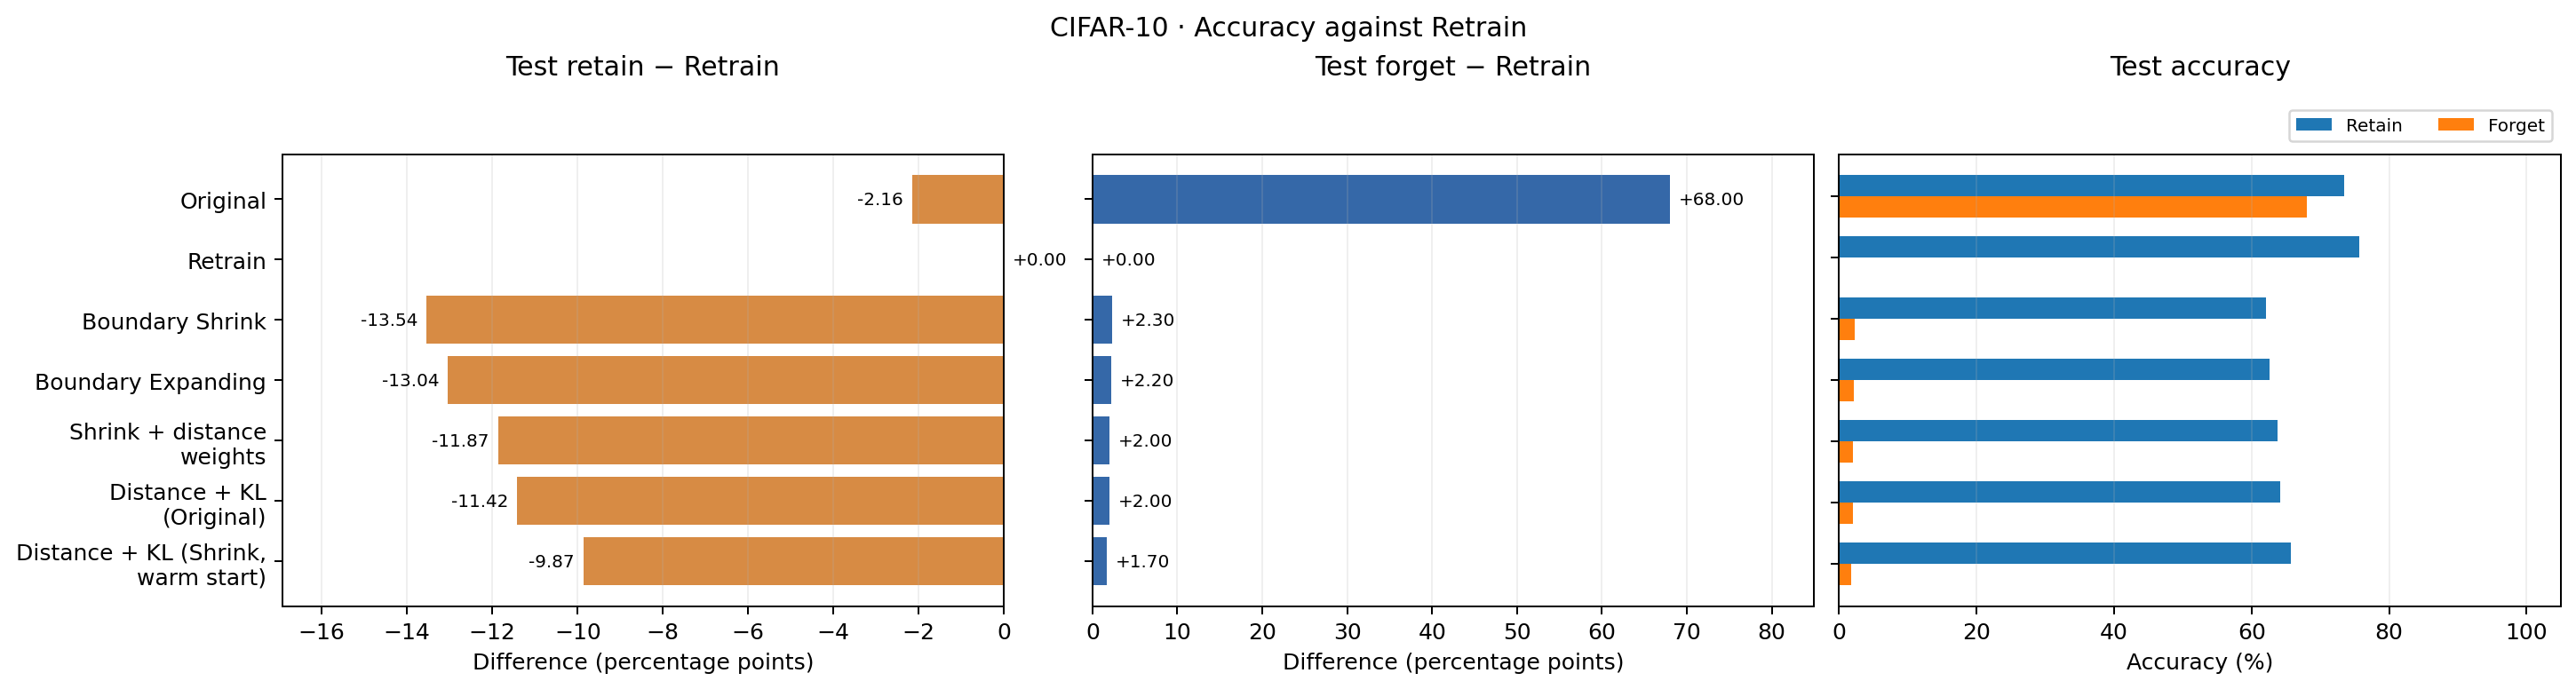
\includegraphics[width=\textwidth]{accuracy.png}
\caption{Test accuracy and differences relative to Retrain on CIFAR-10.}
\label{fig:accuracy}
\end{figure*}
\begin{table}[t]
\centering
\caption{Training and unlearning times of the models on CIFAR-10 and CIFAR-100.}
\label{tab:baseline-cost}
\reporttablefont
\setlength{\tabcolsep}{1.5pt}
\renewcommand{\arraystretch}{1.08}
\begin{tabular*}{\columnwidth}{@{\extracolsep{\fill}}>{\raggedright\arraybackslash}p{0.63in}>{\raggedright\arraybackslash}p{0.84in}*{4}{c}@{}}
\toprule
Dataset & Model & \shortstack{Train\\(s)} & \shortstack{Unlearn\\(s)} & \shortstack{Unlearn\\steps} & Speedup \\
\midrule
CIFAR-10 & Original & 436.18 & --- & --- & ---\\
& Retrain & 399.03 & --- & --- & 1.00\(\times\)\\
& Boundary Shrink & --- & 23.24 & 790 & 17.2\(\times\)\\
& Boundary Expanding & --- & 12.62 & 790 & 31.6\(\times\)\\
\midrule
CIFAR-100 & Original & 424.77 & --- & --- & ---\\
& Retrain & 424.53 & --- & --- & 1.00\(\times\)\\
& Boundary Shrink & --- & 3.18 & 80 & 133.6\(\times\)\\
& Boundary Expanding & --- & 1.44 & 80 & 294.0\(\times\)\\
\bottomrule
\end{tabular*}
\end{table}
Table~\ref{tab:baseline-cost} shows that Boundary Expanding is faster than Boundary Shrink in both runs, consistent with not generating FGSM images for every batch. Both are faster than retraining under the measured settings, but exhibit a utility gap. The CIFAR-100 speedups are obtained with a forget set of 500 images and a budget of 80 updates.

\subsection{Boundary Shrink Variants on CIFAR-10}
\begin{table}[t]
\centering
\caption{Accuracy (\%) of Boundary Shrink, its variants, and Retrain on CIFAR-10.}
\label{tab:variants}
\reporttablefont
\setlength{\tabcolsep}{1.5pt}
\renewcommand{\arraystretch}{1.08}
\begin{tabular*}{\columnwidth}{@{\extracolsep{\fill}}>{\raggedright\arraybackslash}p{0.82in}*{5}{c}@{}}
\toprule
Method & \shortstack{Train\\ret.} & \shortstack{Train\\forg.} & \shortstack{Test\\ret.} & \shortstack{Test\\forg.} & \shortstack{Delta\\Retrain} \\
\midrule
Retrain & 99.70 & 0.00 & 75.61 & 0.00 & 0.00\\
Boundary Shrink & 94.86 & 11.54 & 62.07 & 2.30 & \(-\)13.54\\
DW & 95.76 & 10.12 & 63.74 & 2.00 & \(-\)11.87\\
DW+KL-S & 96.63 & 9.14 & 65.74 & 1.70 & \(-\)9.87\\
\bottomrule
\end{tabular*}
\end{table}
Table~\ref{tab:variants} shows that DW improves test-retain accuracy by 1.67 percentage points over Boundary Shrink. DW+KL-S achieves the highest test-retain accuracy among the evaluated unlearning methods, improving on Boundary Shrink by 3.67 percentage points. Test-forget accuracy decreases from 2.30\% to 1.70\%, corresponding to 17 of the 1,000 deer images still being correctly classified. Nevertheless, this configuration remains 9.87 percentage points below Retrain in test-retain accuracy and retains a train-forget accuracy of 9.14\%.

\begin{table}[t]
\centering
\caption{Execution time and update counts of Boundary Shrink and its variants on CIFAR-10.}
\label{tab:variant-cost}
\reporttablefont
\setlength{\tabcolsep}{1.5pt}
\renewcommand{\arraystretch}{1.08}
\begin{tabular*}{\columnwidth}{@{\extracolsep{\fill}}>{\raggedright\arraybackslash}p{0.70in}*{5}{c}@{}}
\toprule
Method & \shortstack{Final stage\\(s)} & \shortstack{End-to-end\\(s)} & \shortstack{Student\\steps} & \shortstack{Total\\steps} & Speedup \\
\midrule
Boundary Shrink & 23.24 & 23.24 & 790 & 790 & 17.2\(\times\)\\
DW & 94.35 & 94.35 & 790 & 790 & 4.23\(\times\)\\
DW+KL-S & 109.38 & 226.97 & 1,580 & 2,370 & 1.76\(\times\)\\
\bottomrule
\end{tabular*}
\end{table}
The accuracy gains incur a substantial cost (Table~\ref{tab:variant-cost}). DW takes approximately 4.1 times as long as Boundary Shrink with the same 790 updates because it searches over multiple perturbation levels. DW+KL-S requires 109.38 seconds for the final stage and 226.97 seconds in total, including the preparation of DW and Boundary Shrink. The configuration achieving 65.74\% test-retain accuracy provides a speedup of $1.76\times$. Boundary Expanding is the fastest method in the CIFAR-10 run; DW+KL-S achieves the highest test-retain accuracy among the evaluated unlearning methods but uses a larger computational budget.

\subsection{Descriptive Analysis on CIFAR-10}
The supplementary figures in Appendix~\ref{app:visual} use the same models evaluated on CIFAR-10. Grad-CAM uses four train-forget samples with subset indices 355, 2021, 4644, and 1442. The target layer is the final convolutional layer, and the target logit is always deer. The deer probability decreases substantially in these examples after unlearning. The maps show the contribution of each image region to the deer logit; the accompanying predicted label is the class with the highest output probability. Each CAM is independently min--max normalized, showing the relative locations of activation regions within each model. Probabilities in the figures are displayed to one decimal place.

The entropy ECDF uses 2,000 fixed samples from each of the train-retain, train-forget, and test sets. With $H=-\sum_kp_k\ln p_k$, the horizontal axis is $\ln(\max(H,10^{-16}))$, where $H$ is measured in nats. After unlearning, the train-forget curve shifts toward higher entropy, following a trend similar to Retrain. However, the test set contains multiple classes while train-forget contains only deer, so differences also reflect class composition.

The t-SNE analysis uses 1,200 test samples, with 120 samples per class, seed 2022, perplexity 30, and 1,000 iterations. Deer samples are already interspersed with multiple classes in Original. Embeddings are computed separately for each model, producing independent coordinate systems. The qualitative analysis therefore focuses on neighborhood structure within each projection.

% Balance the last two-column page before the one-column appendix.
\balance
\section{Discussion and Limitations}
On both datasets, reducing forgotten-class accuracy is accompanied by a decrease in retained-class accuracy. The unlearning methods have lower computational costs than Retrain but also lower test-retain accuracy, demonstrating a trade-off between execution time and retained-class performance.

On CIFAR-10, the two Boundary Shrink variants improve the metrics relative to the baseline in this run, but the individual contributions of their components have not been isolated. DW simultaneously changes pseudo-labels, attack normalization, and sample weights; DW+KL-S changes initialization, the teacher, and the computational budget. Since these factors change together, the observed differences reflect the effects of the overall configurations.

The experiments use one seed and one forgotten class per dataset. Variability across runs and forgotten classes has not been investigated. On CIFAR-100, the test-forget set contains 100 images, so each image corresponds to one percentage point of accuracy. The study does not use an independent validation set and does not evaluate privacy through membership inference attacks (MIA). The conclusions are therefore limited to the forgotten classes, architecture, and configurations examined.

\section{Conclusion}
This report evaluates the same four models---Original, Retrain, Boundary Shrink, and Boundary Expanding---on CIFAR-10 and CIFAR-100. In both settings, Boundary Shrink and Boundary Expanding reduce forgotten-class accuracy at a lower cost than Retrain while degrading retained-class performance. In the CIFAR-10 experiment, two Boundary Shrink variants improve test-retain accuracy over the baseline. DW+KL-S achieves 65.74\% test-retain accuracy and 1.70\% test-forget accuracy, with a total execution time of 226.97 seconds and a $1.76\times$ speedup over Retrain. DW+KL-S improves retained-class accuracy relative to Boundary Shrink but remains below Retrain and takes longer than the baseline method.

\begin{thebibliography}{10}
\bibitem{bourtoule2021machine}
L. Bourtoule \textit{et al.}, ``Machine Unlearning,'' in \textit{IEEE Symposium on Security and Privacy}, 2021. \url{https://arxiv.org/abs/1912.03817}.
\bibitem{chen2023boundary}
M. Chen, W. Gao, G. Liu, K. Peng, and C. Wang, ``Boundary Unlearning: Rapid Forgetting of Deep Networks via Shifting the Decision Boundary,'' in \textit{CVPR}, 2023, pp. 7766--7775.
\bibitem{golatkar2020eternal}
A. Golatkar, A. Achille, and S. Soatto, ``Eternal Sunshine of the Spotless Net: Selective Forgetting in Deep Networks,'' in \textit{CVPR}, 2020.
\bibitem{goodfellow2015explaining}
I. J. Goodfellow, J. Shlens, and C. Szegedy, ``Explaining and Harnessing Adversarial Examples,'' in \textit{ICLR}, 2015. \url{https://arxiv.org/abs/1412.6572}.
\bibitem{springenberg2015allcnn}
J. T. Springenberg, A. Dosovitskiy, T. Brox, and M. Riedmiller, ``Striving for Simplicity: The All Convolutional Net,'' in \textit{ICLR Workshop}, 2015. \url{https://arxiv.org/abs/1412.6806}.
\bibitem{ioffe2015batch}
S. Ioffe and C. Szegedy, ``Batch Normalization: Accelerating Deep Network Training by Reducing Internal Covariate Shift,'' in \textit{ICML}, 2015, pp. 448--456.
\bibitem{hinton2015distilling}
G. Hinton, O. Vinyals, and J. Dean, ``Distilling the Knowledge in a Neural Network,'' arXiv:1503.02531, 2015.
\bibitem{selvaraju2017gradcam}
R. R. Selvaraju \textit{et al.}, ``Grad-CAM: Visual Explanations from Deep Networks via Gradient-Based Localization,'' in \textit{ICCV}, 2017.
\bibitem{maaten2008tsne}
L. van der Maaten and G. Hinton, ``Visualizing Data using t-SNE,'' \textit{Journal of Machine Learning Research}, vol. 9, pp. 2579--2605, 2008.
\bibitem{krizhevsky2009learning}
A. Krizhevsky, ``Learning Multiple Layers of Features from Tiny Images,'' University of Toronto, Technical Report, 2009. Dataset: \url{https://www.cs.toronto.edu/~kriz/cifar.html}.
\end{thebibliography}
\onecolumn
\nobalance
\appendices
\section{Supplementary Visualizations on CIFAR-10}
\label{app:visual}
The appendix presents Grad-CAM, entropy distributions, and t-SNE visualizations of the models on fixed CIFAR-10 samples.
\begin{figure}[!ht]
\centering
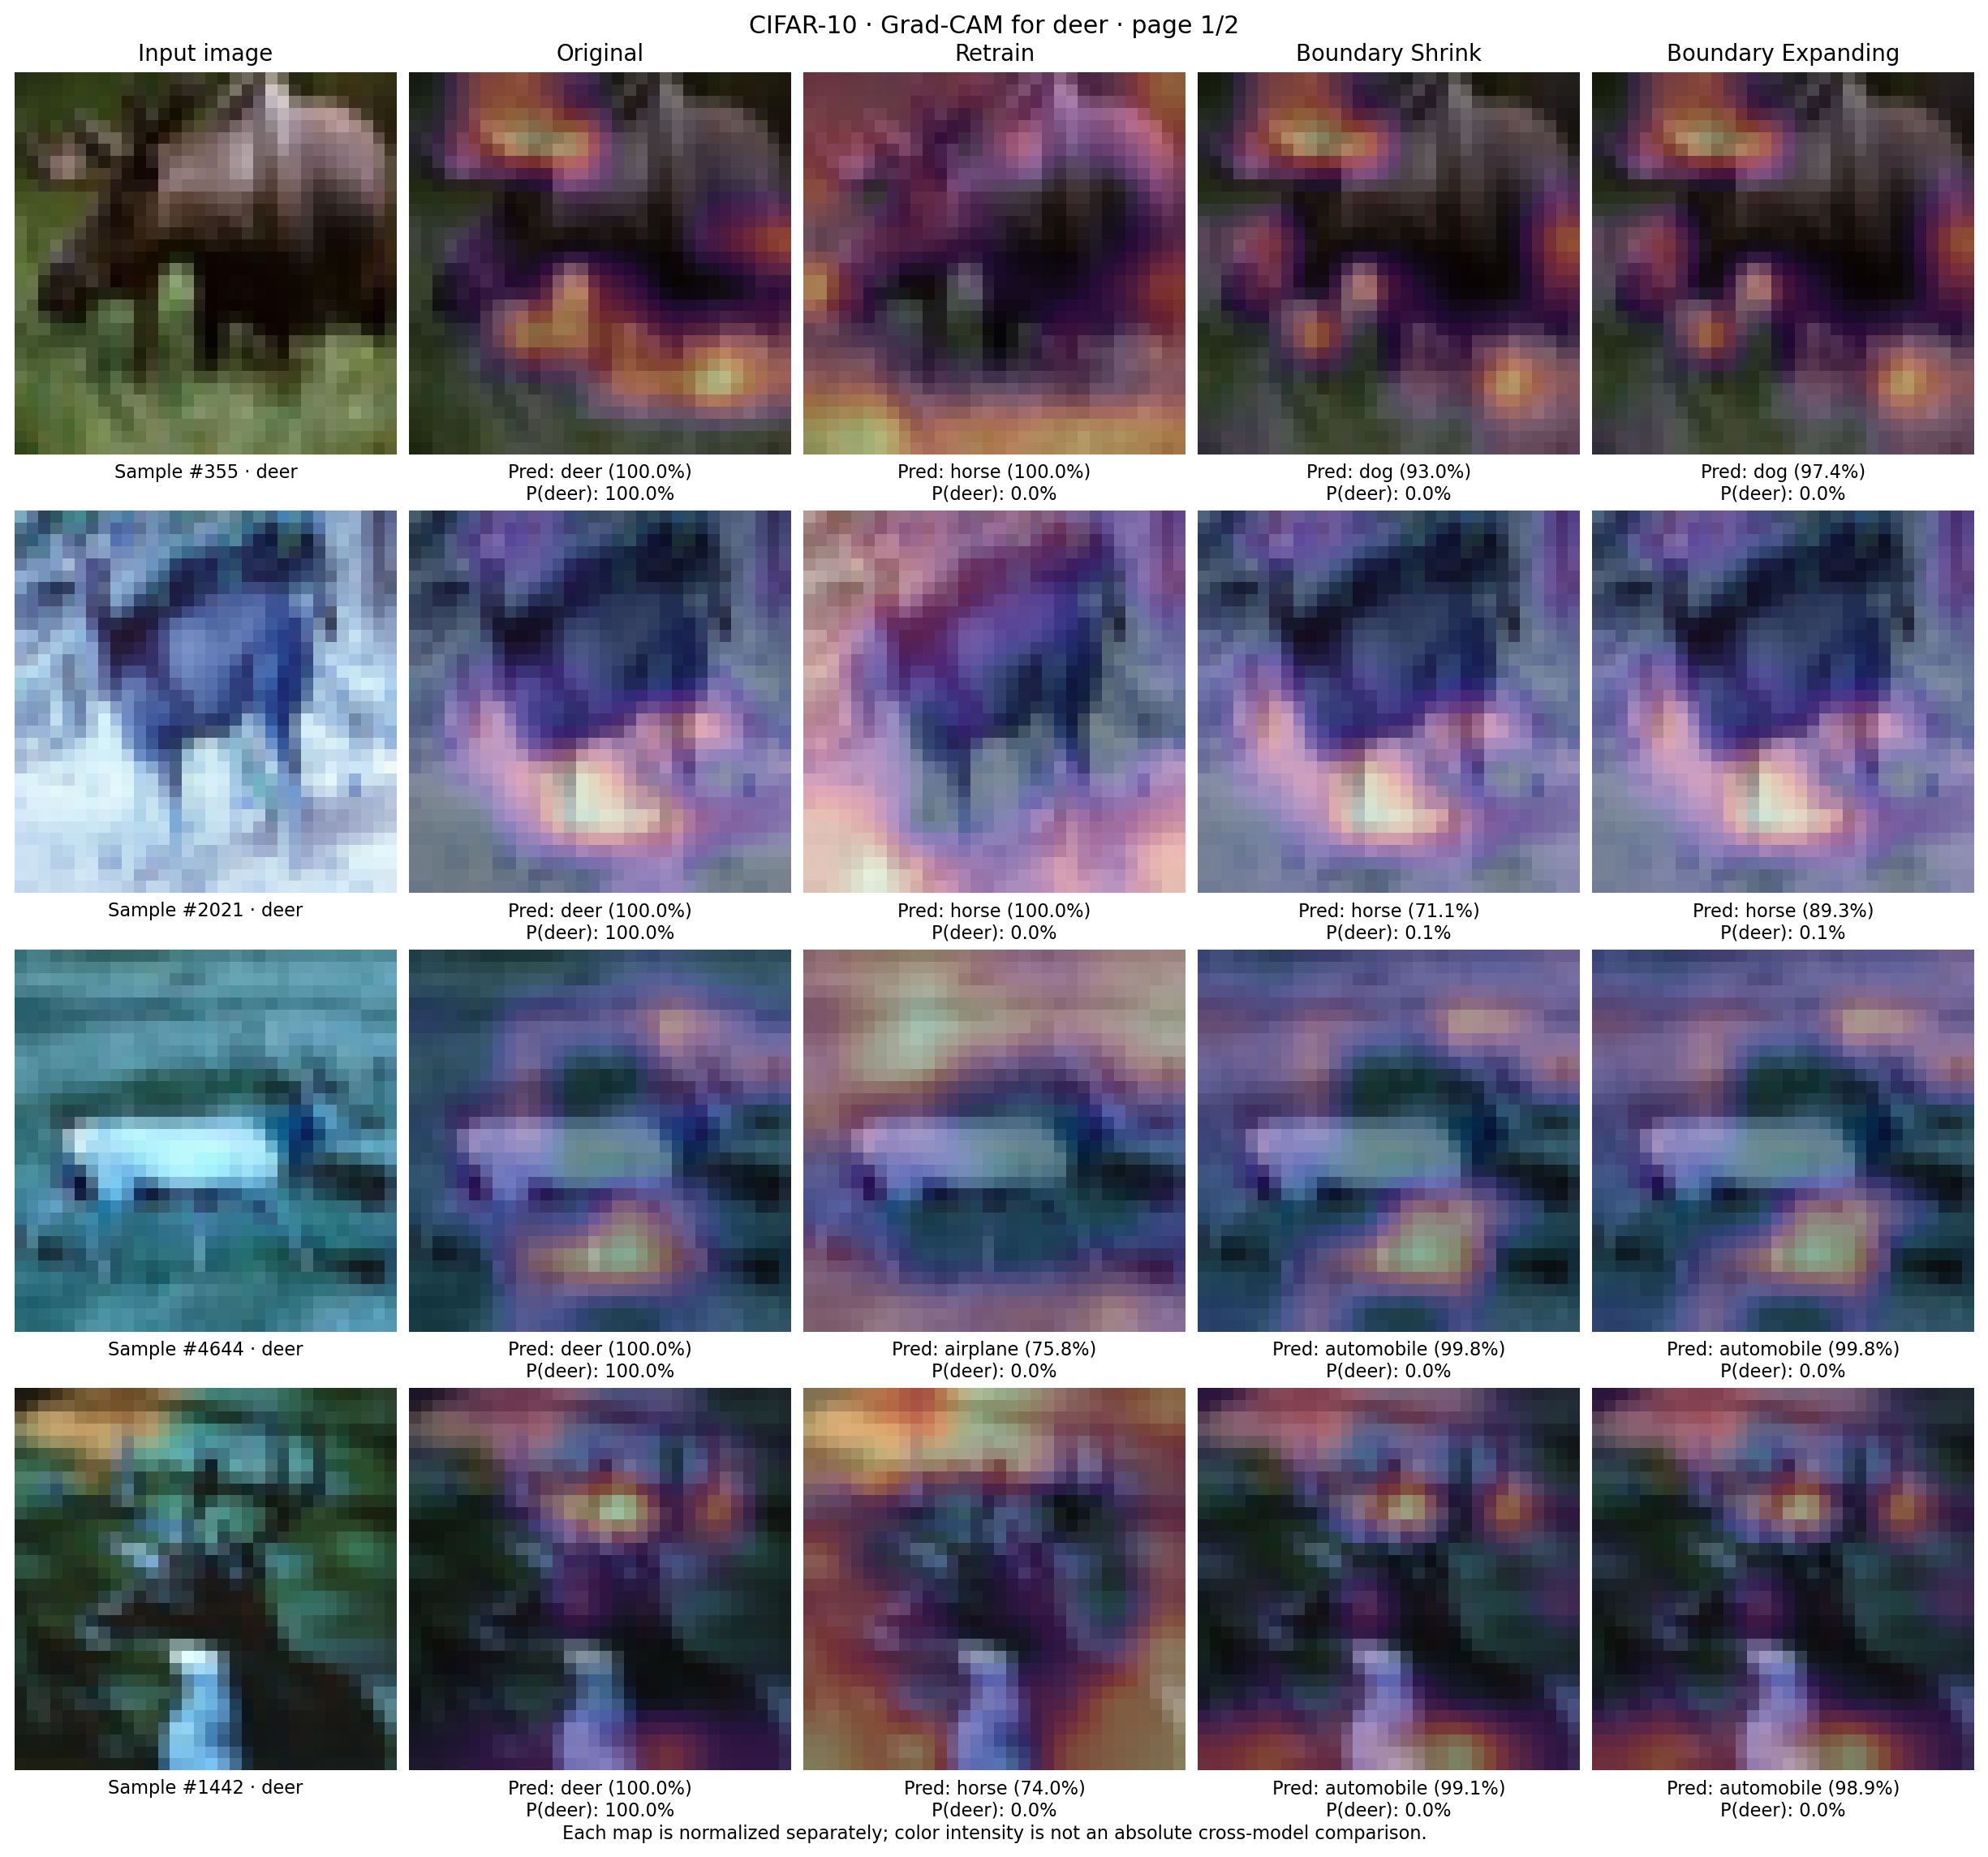
\includegraphics[width=0.94\textwidth,height=0.70\textheight,keepaspectratio]{gradcam_1.png}
\caption{Grad-CAM for the deer logit of Original, Retrain, Boundary Shrink, and Boundary Expanding on four CIFAR-10 train-forget samples.}
\label{fig:cam-base}
\end{figure}
\clearpage
\begin{figure}[!ht]
\centering
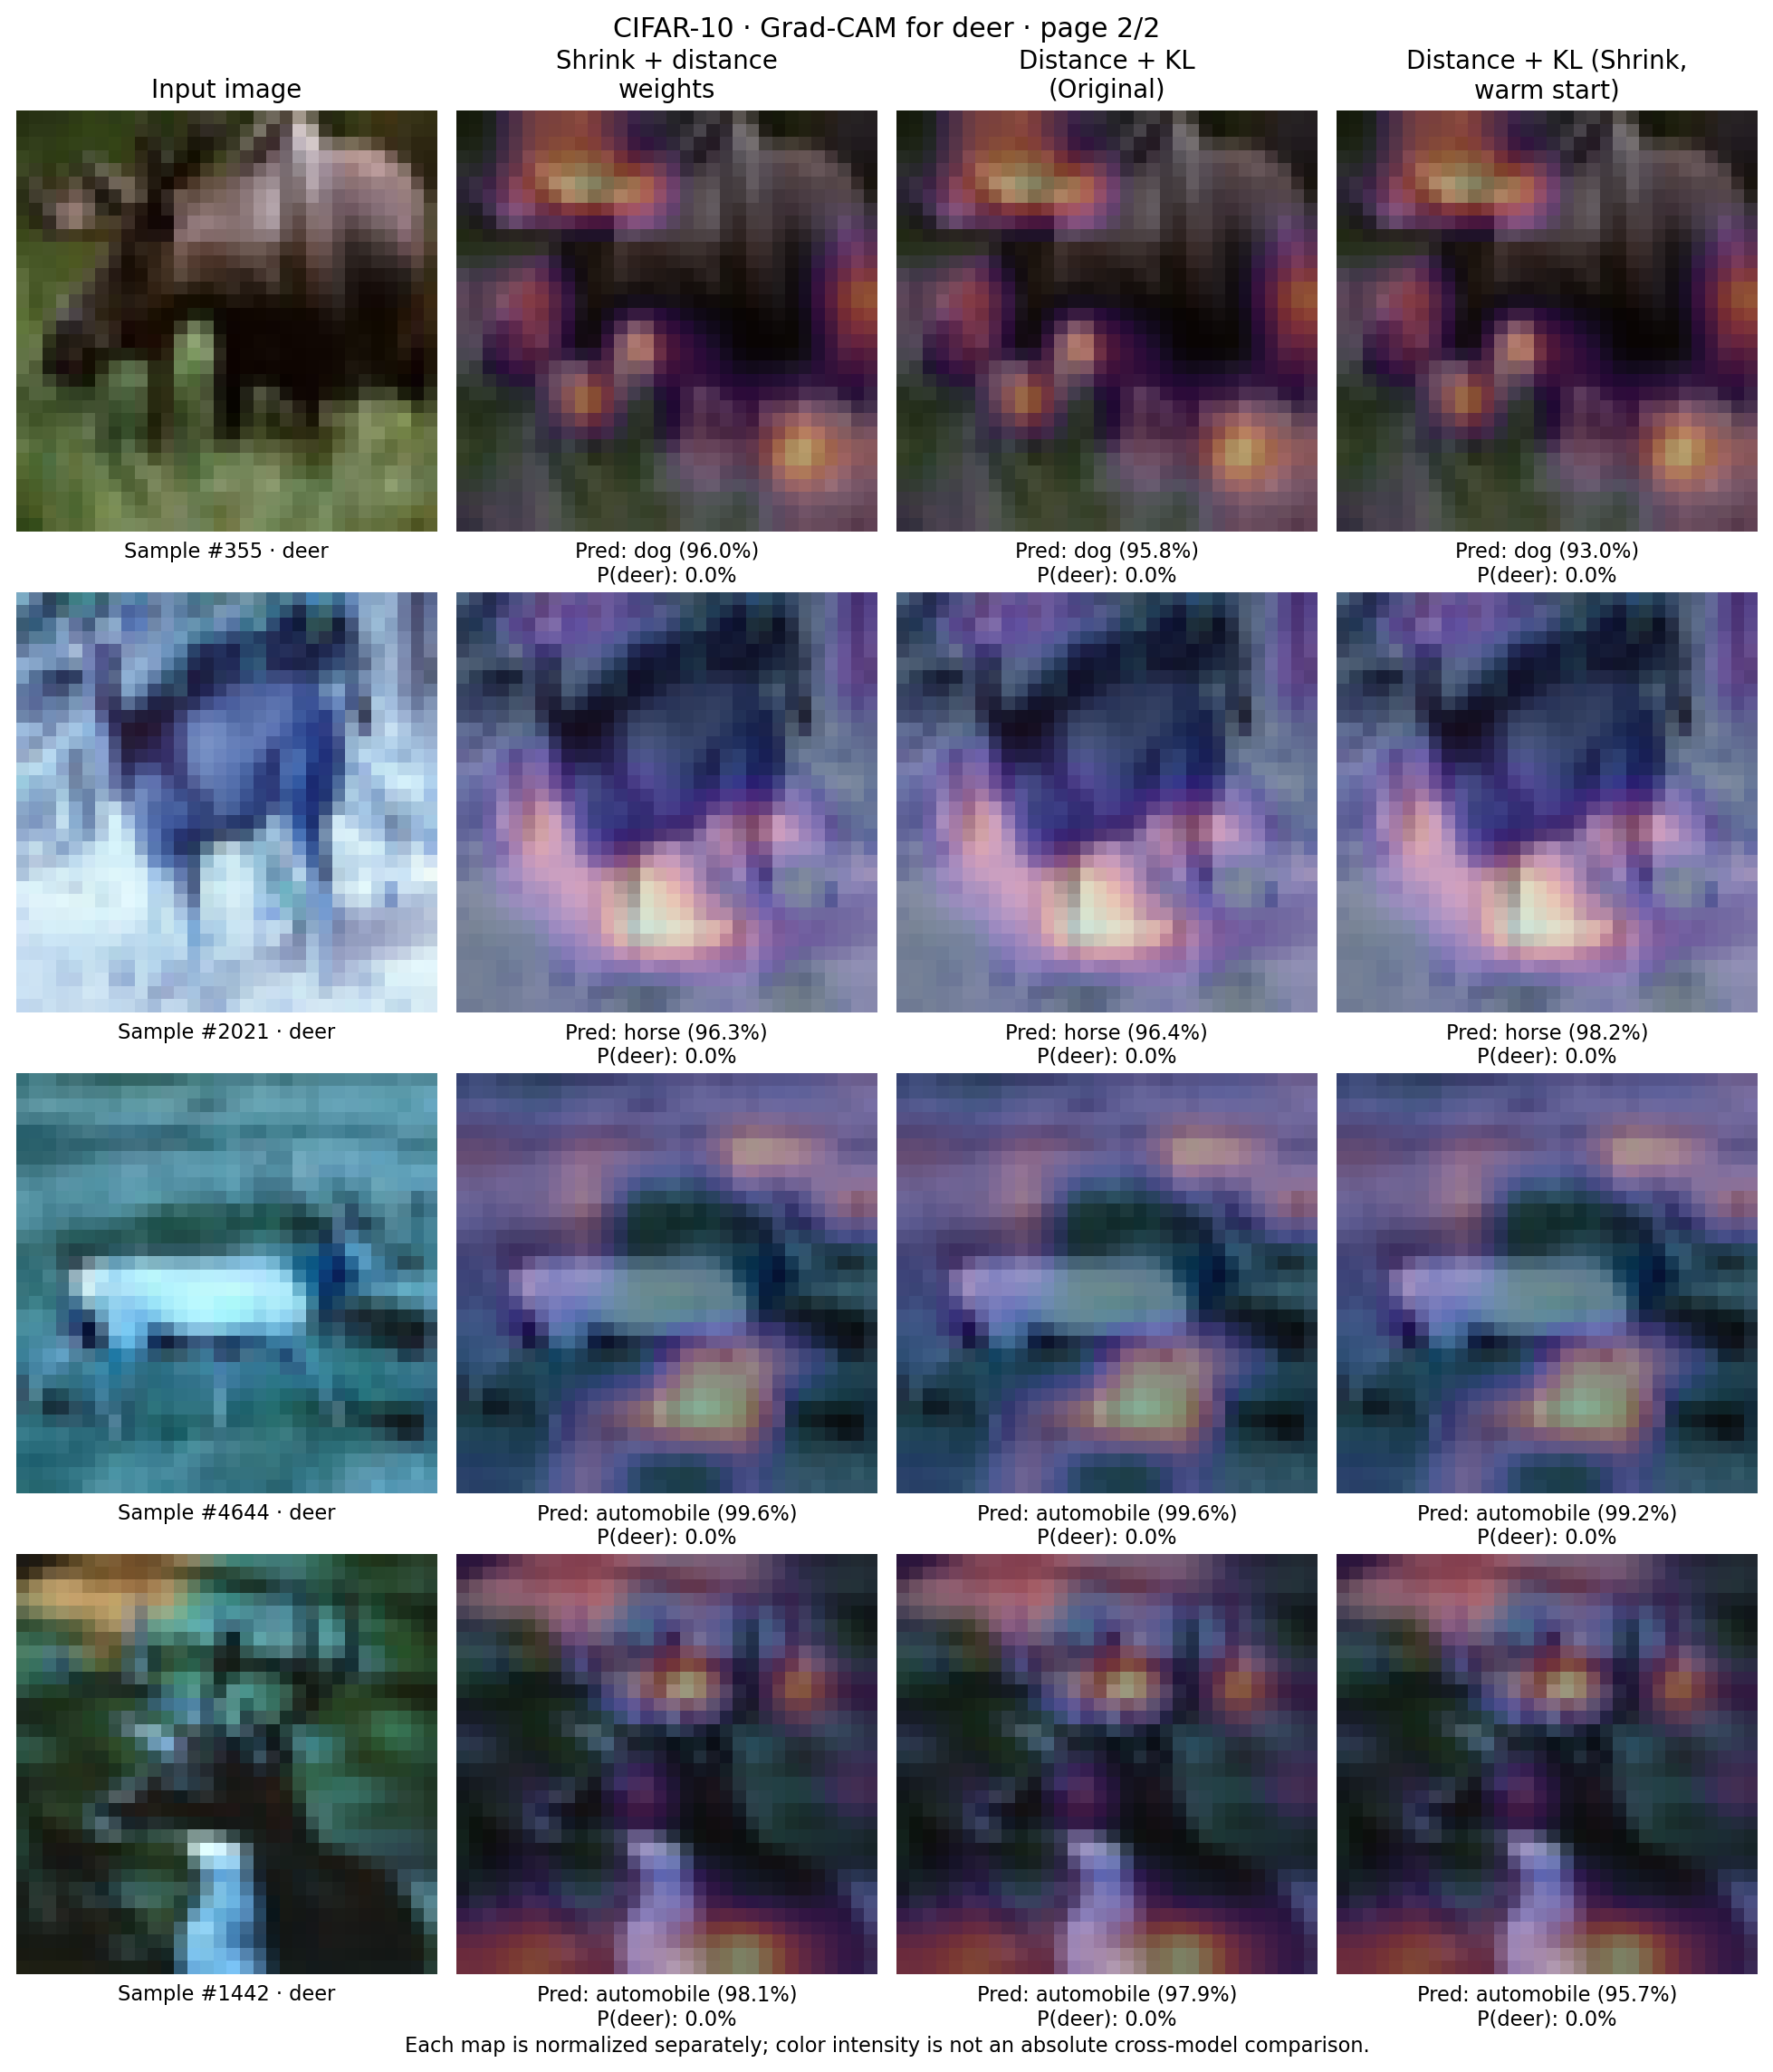
\includegraphics[width=0.84\textwidth,height=0.70\textheight,keepaspectratio]{gradcam_2.png}
\caption{Grad-CAM for the deer logit of the Boundary Shrink variants on the same four CIFAR-10 train-forget samples.}
\label{fig:cam-variants}
\end{figure}
\clearpage
\begin{figure}[!ht]
\centering
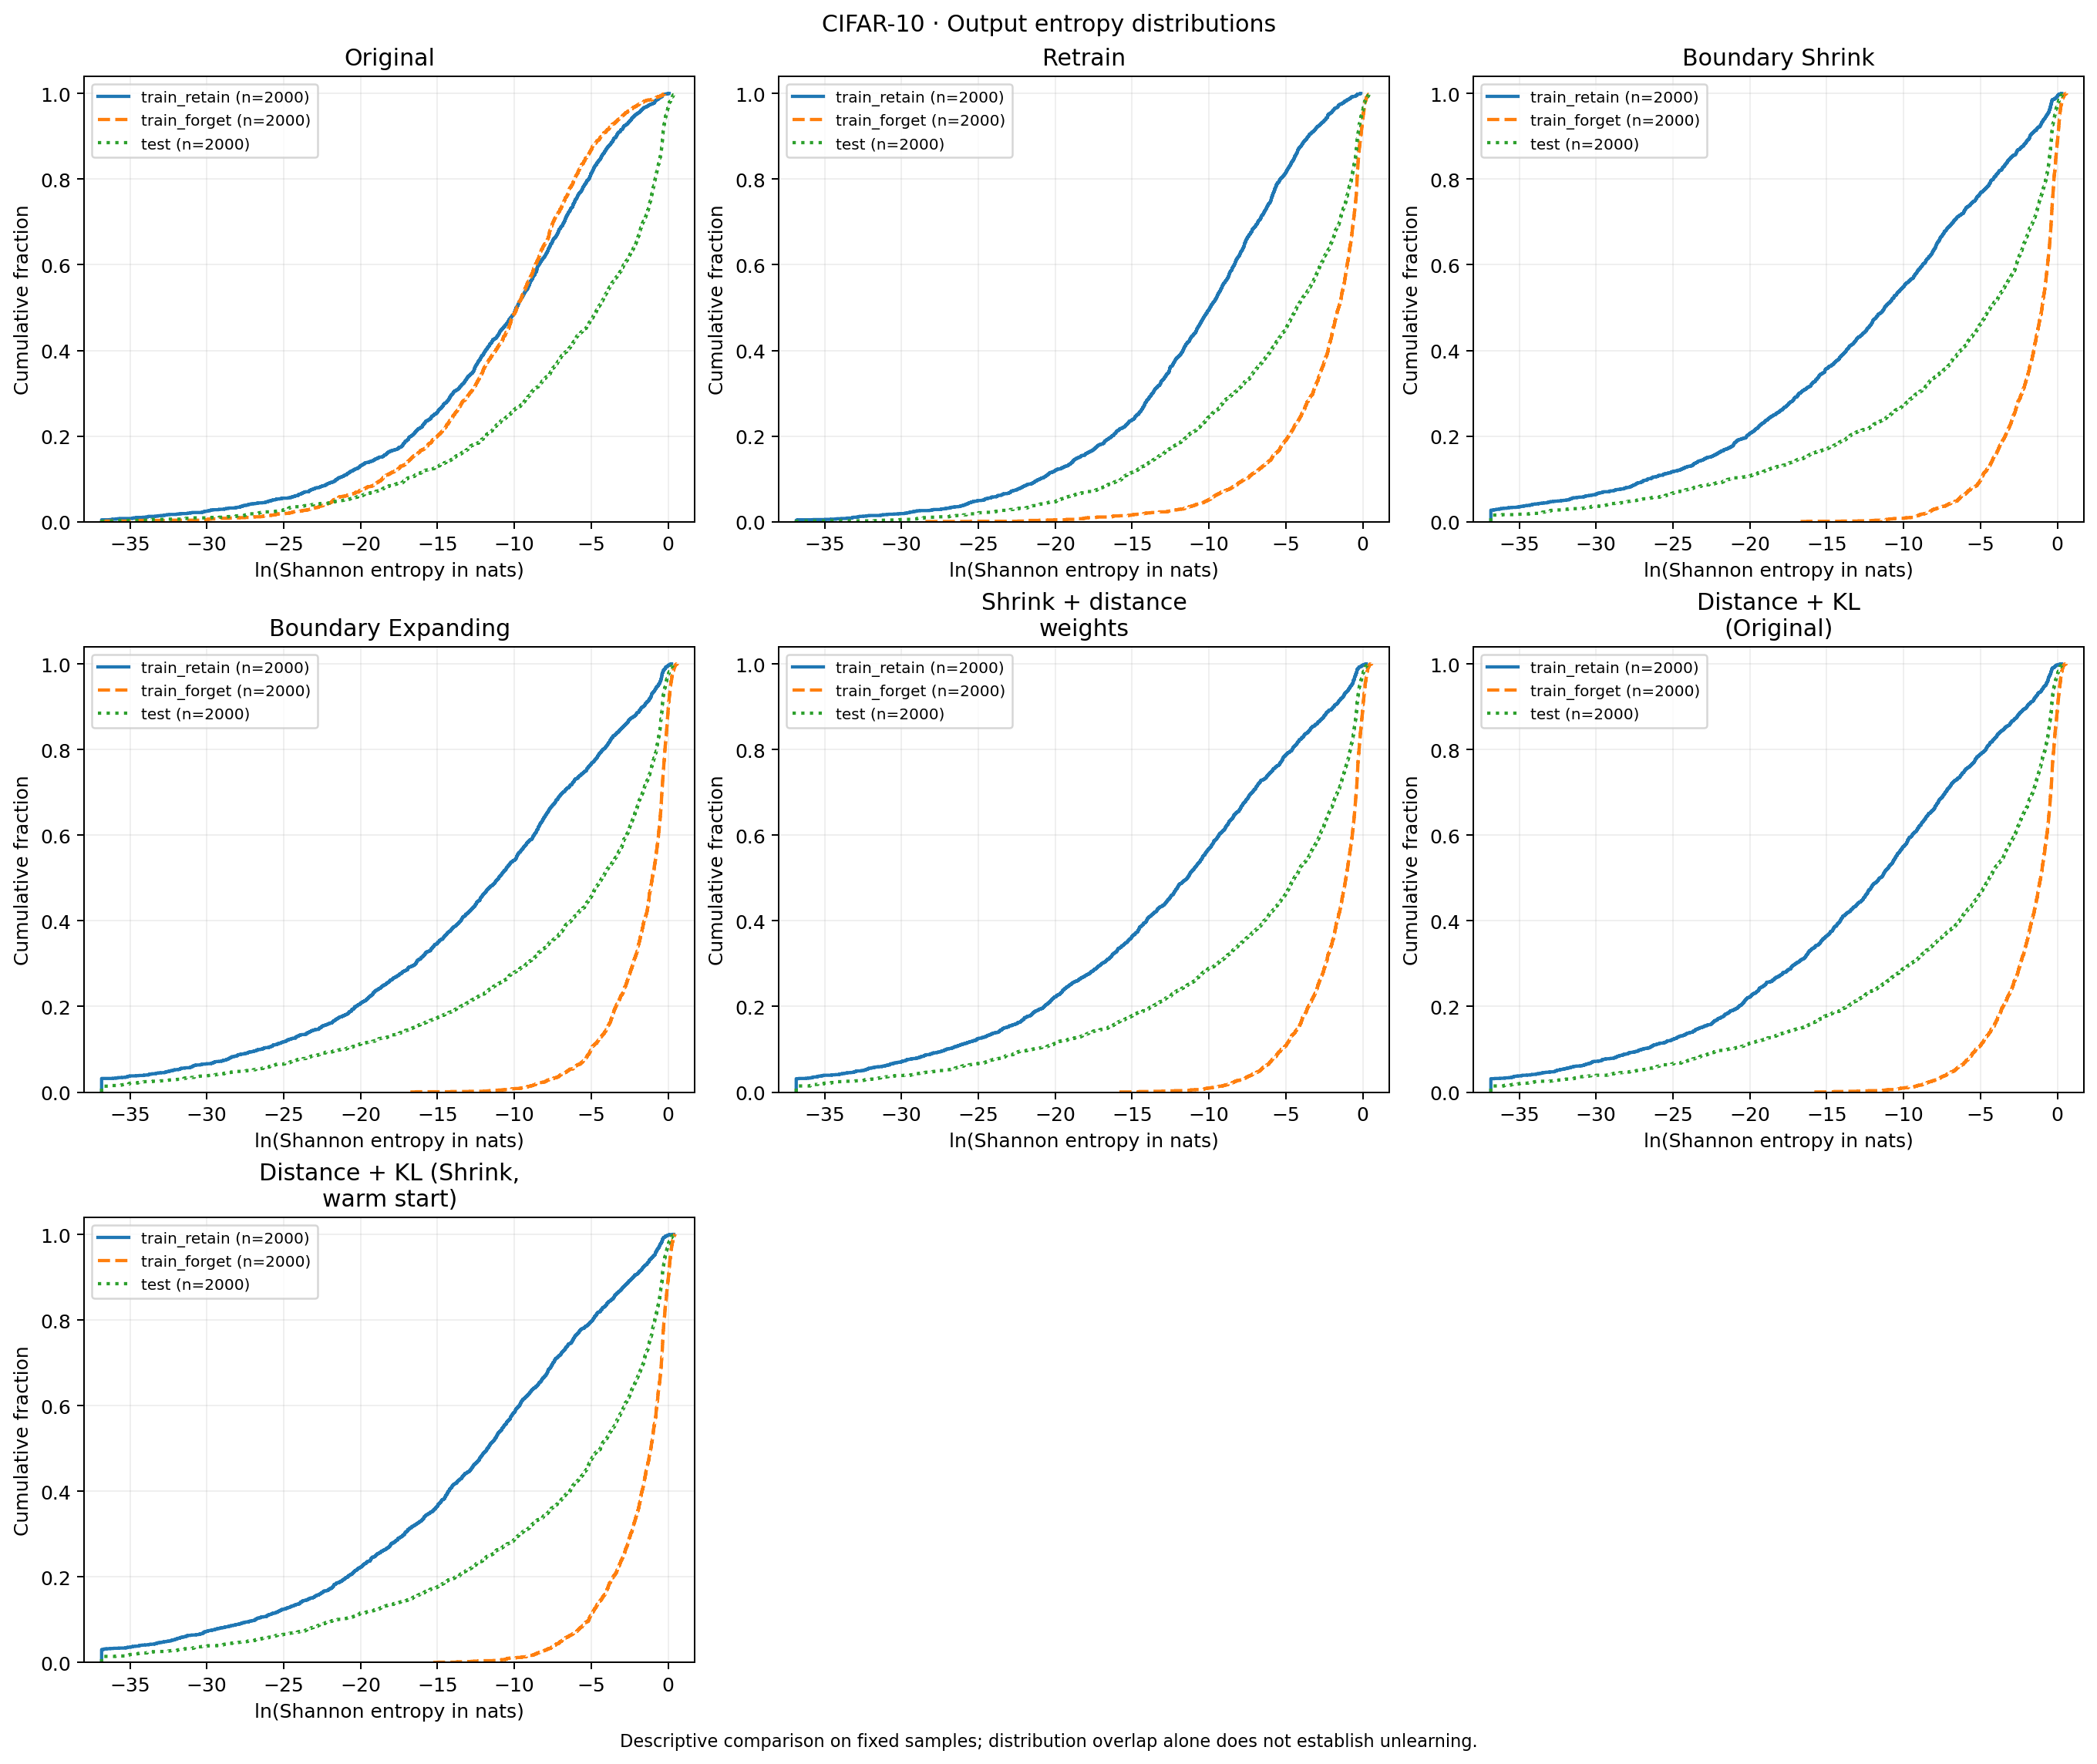
\includegraphics[width=1\textwidth,height=0.76\textheight,keepaspectratio]{entropy.png}
\caption{Empirical cumulative distributions of log entropy on the CIFAR-10 train-retain, train-forget, and test sets (2,000 samples per set).}
\label{fig:entropy}
\end{figure}
\clearpage
\begin{figure}[!ht]
\centering
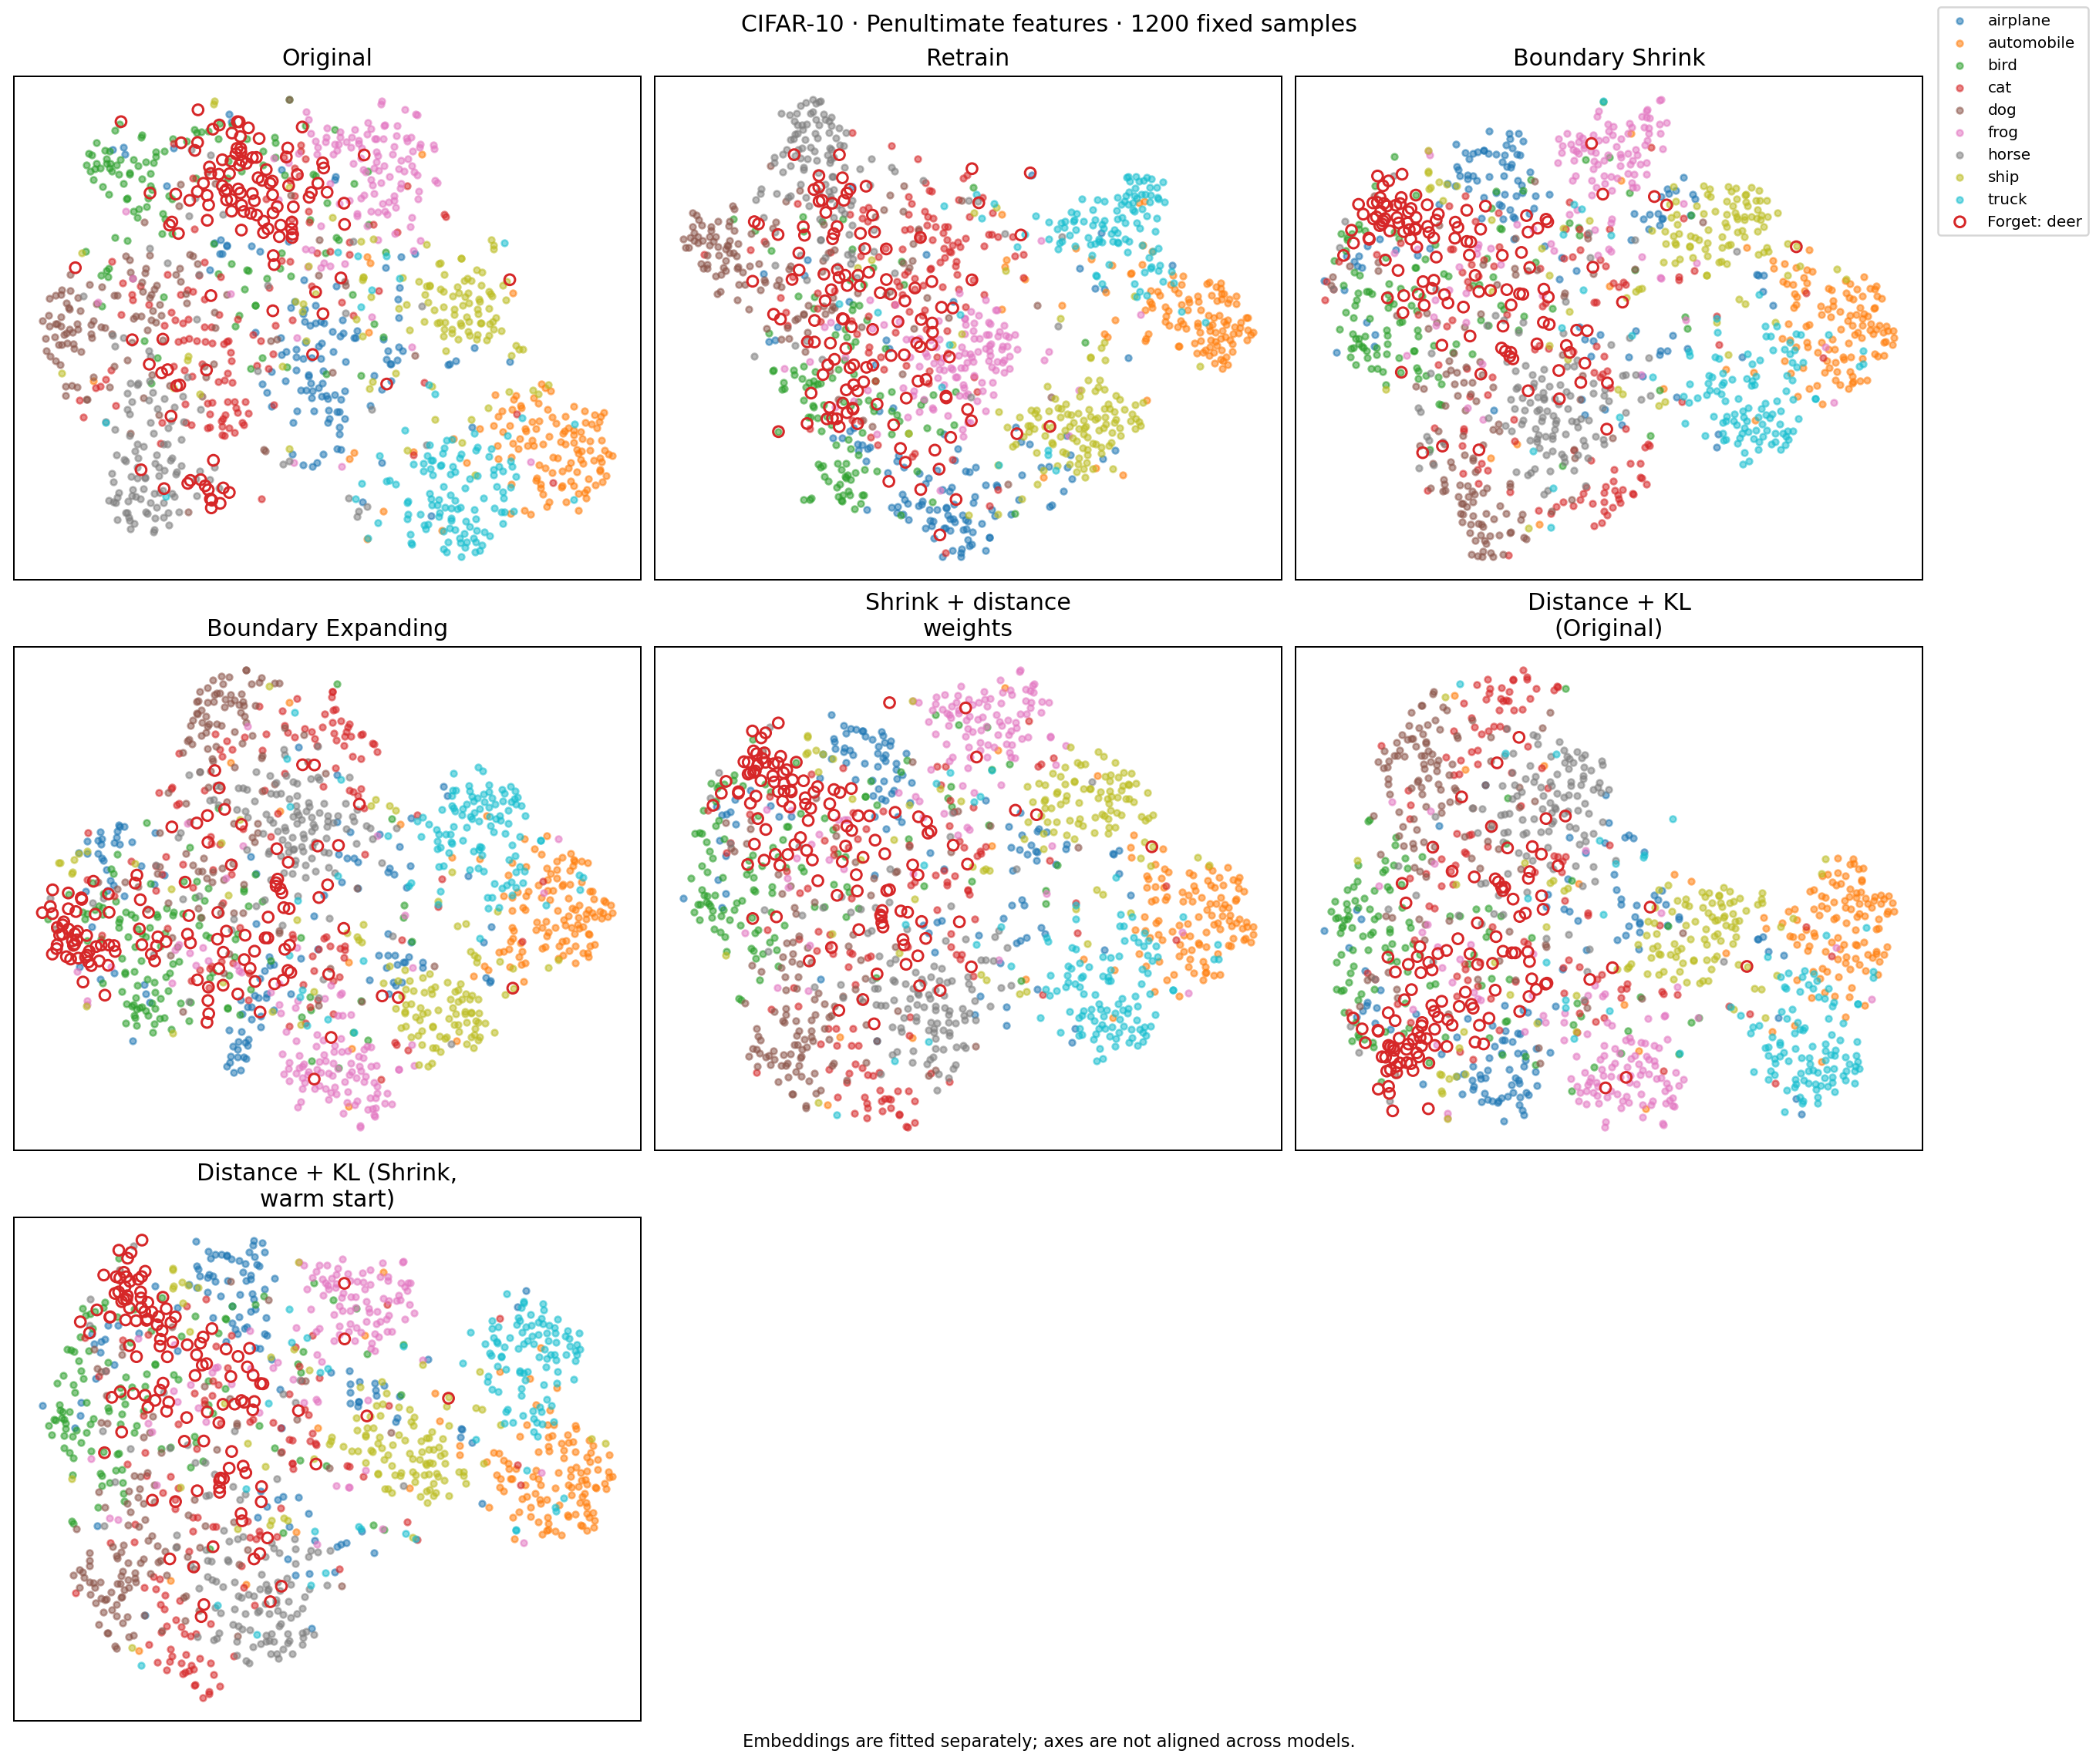
\includegraphics[width=1\textwidth,height=0.76\textheight,keepaspectratio]{tsne.png}
\caption{t-SNE representations of 1,200 CIFAR-10 test samples, with 120 samples per class; hollow circles denote the deer class.}
\label{fig:tsne}
\end{figure}
\end{document}
